\documentclass[../../../main.tex]{subfiles}
\begin{document}
\begin{minipage}{\textwidth}
	\begin{center}
		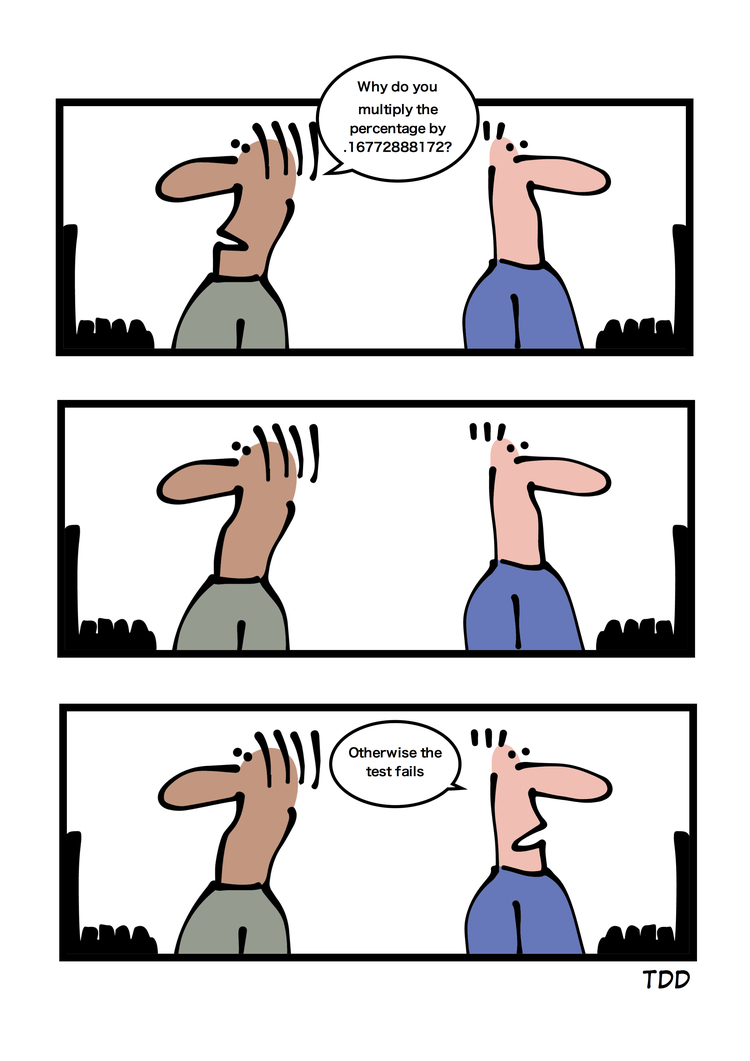
\includegraphics[width=0.4\textwidth]{meme1}
	\end{center}
\end{minipage}

La gestion d'erreurs en programmation est absolument fondamentale. Les raisons sont multiples :
\begin{itemize}
	\item un ordinateur physique n'est pas théorique, et un programme subit tous les défauts de l'implantation.
On peut par exemple penser aux opérations sur les nombres flottants qui induisent une imprécision.
Les résultats obtenues sur les flottants sont donc dans la majorité des cas faux pour la modélisation
de nombres réels
	\item les programmes développés sur un ordinateur ont été écrits par des humaines faillibles. Ainsi, il
n'est jamais sûr à 100\% qu'un programme écrit soit correct, bien qu'il soit démontré correct en
théorie.
\end{itemize}
Bien sûr, dans le cas de ``petits'' programmes, ne pas gérer les erreurs n'a qu'une incidence minime sur
le développement. Dans le cas de très grands projets, des erreurs humaines ont de fortes chances de
se glisser dans certaines étapes du développement et les tester et les gérer est extrêmement important
pour éviter des bogues incontrôlés et surtout non localisés.

Les manquements à la gestion des erreurs et aux tests sont la source première des failles de sécurité
des systèmes informatiques.\footnote{Le test logiciel fait malgré tout partie (de mon point de vue subjectif) des domaines de l'informatique pratique les plus atrocement chiants dont j'ai pu faire l'expérience\dots Je veux dire par chiant : un ennui morbide qui fabrique des boules de déprime calées devant des écrans à se demander toutes les cinq secondes l'heure qu'il est \dots Et le pire, c'est l'automatisation de tests logiciels en PowerShell sous Windows. Ça c'est particulièrement horrible.}
\subsection{Un petit exemple pour prendre la température}
Lorsque l'on commence à programmer, en C notamment, les erreurs de segmentation sont parmis
les plus fréquentes.\footnote{Ah bon ?} Pour les réduire, il faut au maximum réduire les probabilités de manipuler des
pointeurs non initialisés. Pour cela, il faudrait tester après chaque initialisation de pointeur (par un
malloc par exemple) si le pointeur est effectivement non \textsf{NULL}.

Avec un malloc cela ressemblerait à :
\begin{minted}[linenos=false]{c}
int *x = NULL;
x = (int *)malloc(10 * sizeof(int));
if (!x) {
	fprintf(stderr, "Erreur d'allocation memoire !\n");
}
\end{minted}
En toute rigueur, c'est ce qu'il faudrait faire. En effet, si l'ordinateur ne dispose plus d'assez de mémoire
vive pour allouer dynamiquement la variable, malloc renverra \textsf{NULL}. Dans les faits, effectuer un test à
chaque allocation est assez lent. Si on sait qu'on alloue pas 3 ou 4 \textit{Go} d'un coup, la probabilité d'erreur
est furieusement proche de zéro. Et si le système d'exploitation n'arrive pas à allouer une centaine
d'octets dynamiquement, il y a fort à parier qu'il ne puisse rien faire du tout de toute manière et
qu'une erreur de segmentation n'ait aucune incidence dans la pratique.

\textbf{Remarque :} Dans le cas de la programmation de systèmes embarqués, le paragraphe précédent
est nul et non avenu puisque les systèmes embarqués doivent fonctionner avec des ressources parfois
extrêmement limités. La question est alors plus de trouver une autre manière de faire qui optimise la
quantité de mémoire utilisée.

La gestion des erreurs est donc dépendante du contexte.
\subsection{Codes d'erreur}
Les routines de la bibliothèque standard du langage C renvoient une valeur indiquant le comportement
de l'exécution de ladite routine. Ainsi, il est possible de contrôler le bon fonctionnement d'un grand nombre de fonctions de la bibliothèque standard.

Par exemple, l'ouverture d'un fichier grâce à \textsf{fopen} peut échouer car il n'existe pas de fichier accessible
par le chemin indiqué ou encore car un autre programme utilise déjà ce fichier. Le test :
\begin{minted}[linenos=false]{c}
const char* filename = ...;
FILE *fd = fopen(filename, "mode");
if (!fd) {
	fprintf(stderr, "Erreur d'ouverture du fichier %s\n", filename);
} else {
	...
}
\end{minted}
permet d'effectuer le contrôle de la bon ouverture du fichier. En effet, \textsf{fopen} renvoie \textsf{NULL} si la fonction
échoue.

La gestion d'erreur dépend de chaque fonction. Ainsi, les fonctions \textsf{fread} et \textsf{fwrite} renvoient le nombre
de caractères lues ou écrits. C'est donc en contrôlant ce nombre que l'on sait si la fonction a échoué.
La lecture du manuel est ici indispensable.
\end{document}